\section{Taking a slice: diabetic patient analysis}\label{sec:diabetes}

The main conclusion to be taken away from the previous summative analysis is
that the dataset contains a huge amount of variation. Therefore, in order to
conduct more meaningful analysis, more homogenous subsets of the data must be
considered.

Classically, patients are categorised by age or condition~\cite{Vuik2016}. In
this section, the focus will be on the diabetic population within the dataset.
Since diabetes is recorded only as a primary or secondary condition in the
dataset and is not distinguished by type, the diabetic population is considered
to be any instance where diabetes is present.

The ensuing analysis will provide evidence that the diabetic population is
increasing in the Cwm Taf area, and that, despite this, the relative resource
consumption by diabetic patients has been stagnant over the data period. It will
also be seen that this population holds too much variation to make meaningful 
conclusions about the population on the whole. However, by considering a subset
based on a condition such as this, there is a natural opportunity to compare
the subset with its complement; by considering the differences and similarities
between these two datasets a new dimension is added to the analysis.


\subsection{Distributions}\label{subsec:diabetes_dists}

\begin{itemize}
    \item All the plots in the same order as previous section
    \item Summary for each plot and comparison where applicable
\end{itemize}


\begin{figure}[htbp]
    \centering
    \includegraphics[width=\imgwidth]{no_spells_bar/main.pdf}
    \caption{Bar chart for the number of spells associated with a patient in the
        presence of diabetes and not.}%
    \label{fig:diabetes_no_spells_bar}
\end{figure}

\begin{figure}[htbp]
    \includegraphics[width=\imgwidth]{los_bar/main.pdf}
    \caption{Bar chart for the total length of a spell in the presence of
        diabetes and not, clipped at 21 days.}%
    \label{fig:diabetes_los_bar}
\end{figure}

\begin{figure}[htbp]
    \centering
    \includegraphics[width=\imgwidth]{no_diag_bar/main.pdf}
    \caption{Bar chart for the maximum number of diagnoses in a spell in the
        presence of diabetes and not.}%
    \label{fig:diabetes_no_diag_bar}
\end{figure}

\begin{figure}[htbp]
    \centering
    \includegraphics[width=\imgwidth]{no_proc_bar/main.pdf}
    \caption{Bar chart for the total number of procedures in a spell in the
        presence of diabetes and not.}%
    \label{fig:diabetes_no_proc_bar}
\end{figure}

\begin{figure}[htbp]
    \centering
    \includegraphics[width=\imgwidth]{netcost_kde/main.pdf}
    \caption{Estimated probability density for the net cost of a spell in the
        presence of diabetes and not, clipped at \pounds12,500.}%
    \label{fig:diabetes_netcost_kde}
\end{figure}


\subsection{Pairwise correlation}\label{subsec:diabetes_correlation}

\begin{itemize}
    \item Correlation heatmap
    \item Ordering is based on diabetic population now \-- any changes?
    \item Differences heatmap
\end{itemize}


\subsection{Variation and relative importance}\label{subsec:diabetes_variation}

\begin{itemize}
    \item Variation/contribution plots \-- ordering same as above
    \item Bubble plot
    \item Conclusions
\end{itemize}
